% !TEX root = ./cvl.tex
\section{Algorithms for single-scale filtering}
\label{sec:algorithms}

The algorithmic framework for the multi-scale filtering problem is illustrated in Figure~\ref{fig:algorithmic-framework}. After an initialization step, we solve $\mathcal{Z}$ single-scale filtering problems --- followed by a finalizing step.

\marcos{The algorithmic framework is not for multi-scale filtering, but for iterated single-scale filtering? Seems to me that these two are not the same thing.}

\begin{figure}[htbp]
\begin{center}
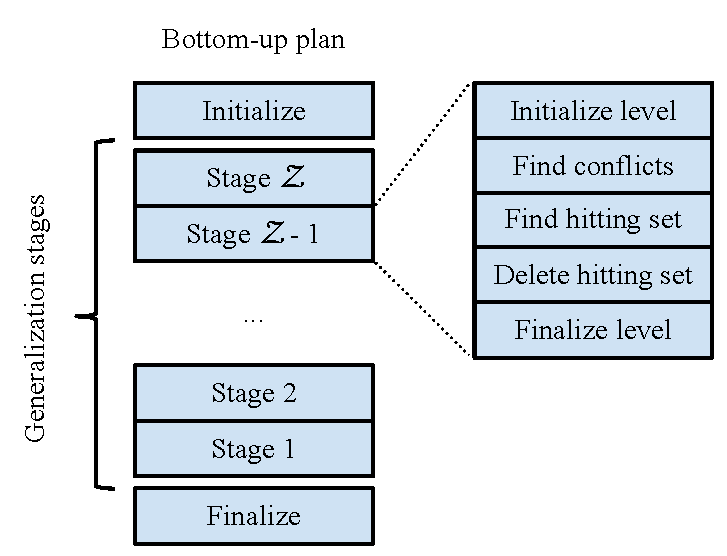
\includegraphics[scale=.6]{figs/cvl_stages.pdf}
\caption{The algorithmic framework: At stage $i$ the single-scale filtering problem is solved for the $i'th$ zoom level.}
\label{fig:algorithmic-framework}
\end{center}
\end{figure}

Below we describe two different heuristic algorithms for solving the single-scale optimization problem. Let $n=|\bar{C}|$ be the number of conflict sets (or elements in the set multicover problem), and let $m=|\bar{R}|$ be the number of records (or sets in the set multicover problem). Recall that $\bar{R}_c \subseteq \bar{R}$ is the set of records in conflict set $c \in \bar{C}$. The largest number of records in any conflict set is $f = \max_{c \in \bar{C}} |\bar{R}_c|$, and is called the \emph{maximum frequency}.

\subsection{Static greedy algorithm (SGA)}
\label{sec:algorithms:sga}

In this algorithm we consider each conflict set $c \in \bar{C}$ in turn, and simply choose the $\lambda_c$ records with minimum weight from conflict set $\bar{R}_c$ --- independently of what has been chosen earlier. If the sets $\bar{R}_c$ are disjoint, the algorithm is clearly optimal. However, in general no approximation guarantee can be provided. The algorithm runs in $O(n f \log f)$ time, as we just need to sort the records by weight for each conflict set; alternatively we can sort all records by weight in $O(m \log m)$ time and pick the minimum weight records from the conflict sets in linear time in the total number of records in all conflict sets.

%\kostas{we should revisit our use of constraint and conflict set. in the SGA we are sorting each conflict set, not each constraint.}
%\martin{Done}

\subsection{LP-based greedy algorithm (LPGA)}
\label{sec:algorithms:lpga}

In this algorithm we first solve a linear programming (LP) relaxation of the set multicover problem. This LP-problem is obtained by relaxing the constraint $x_r \in \{0, 1\}$ to $0 \leq x_r \leq 1$. Then we choose all records $r \in \bar{R}$ for which the LP-solution variable $x_r$ is at least $1 / f$. Intuitively, we round up to 1 all fractional values that are large enough; the remaining fractional variables are rounded down to 0. 

This algorithm provides a feasible solution to the single-scale problem, and the approximation guarantee is $f$~\cite{vazirani2001approximation}; thus, if $f$ is small, the algorithm provides a good approximation guarantee. As the LP-problem can be solved in polynomial time, the complete algorithm is polynomial.

%\subsection{Dynamic greedy algorithm (DGA)}

%Described in Vazirani 13.2.1. @Martin: Please write here.

%\marcos{I would only introduce DGA if it is actually evaluated in the experiments.}

